\begin{figure}[t!]
\begin{center}
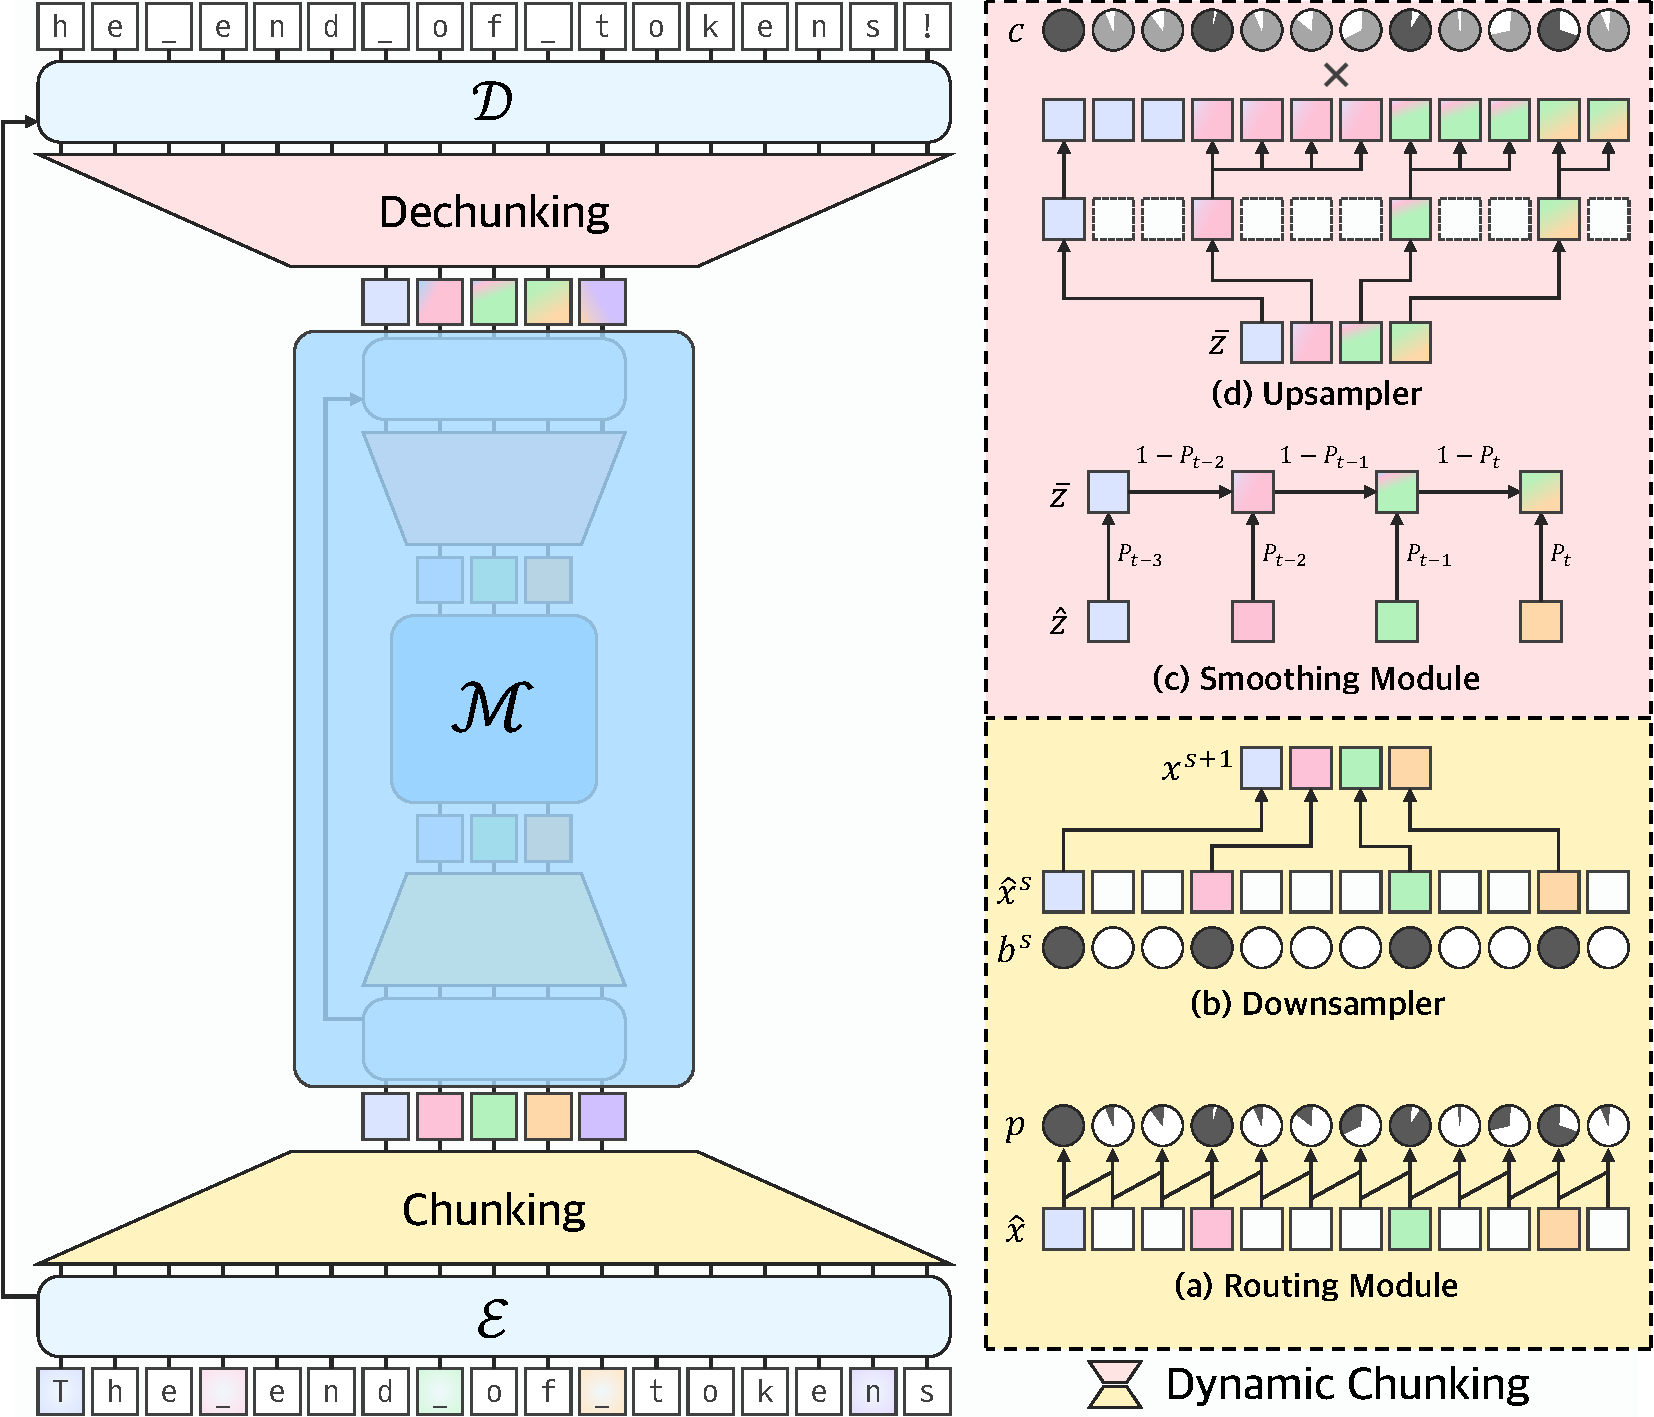
\includegraphics[width=\linewidth]{fig_img/main.pdf}
\end{center}
\caption{
\textbf{(left)} Architectural overview of H-Net with a two-stage hierarchical design ($S=2$).
\textbf{(right)} Dynamic Chunking (DC).
\textbf{(\colorbox{Chunk}{bottom-right})} Key components of a \chunk{}:
(a) a \router{} for dynamically drawing chunk boundaries, and
(b) a \downsampler{} that selectively retains vectors based on boundary indicators, reducing sequence length while preserving semantically significant positions.
\textbf{(\colorbox{DeChunk}{top-right})} Key components of a \dechunk{}:
(c) a \smoother{} for converting discrete chunks into interpolated representations, and
(d) an \upsampler{} that restores compressed vectors to their original resolution based on boundary indicators.
$\mathsf{Linear}$ in equation \eqref{eq: detokenizer} and $\mathsf{STE}$ in equation \eqref{eq: Upsampler-Mult} are omitted in the illustration for brevity.
}
\label{fig: main}
\end{figure}